\title{Лекция 14\\Основные принципы разработки семантических моделей баз знаний}
\author[]{Шункевич Д.В.}
\institute[]{Белорусский государственный университет информатики и радиоэлектроники}

\begin{frame}
	\titlepage
\end{frame}

\begin{frame}{\\Содержание лекции}
	\topline
	\justifying
	Методика разработки баз знаний, основные этапы. Выделение иерархии предметных областей. Формирование онтологий.
\end{frame}

\begin{frame}{Методика разработки баз знаний}
	\topline
	\justifying 

	В современной литературе при анализе методов разработки баз знаний основное внимание уделяется анализу методологий разработки \textbf{\textit{онтологий}}, которые являются основной частью современных баз знаний.
 
    Методология разработки онтологий представляет собой набор инструкций и руководств, описывающих процесс выполнения сложных процедур разработки онтологий. Она детализирует различные задачи, как они должны быть выполнены, в каком порядке и каким образом осуществлять документирование работы по созданию онтологий.
    
\end{frame}

\begin{frame}{Основные этапы разработки гибридных баз знаний}
	\topline
	\justifying
	\vspace{8mm}
	\begin{textitemize}
		\item Формирование начальной структуры гибридной базы знаний.
		\item Выявление компонентов базы знаний, которые могут быть заимствованы из библиотеки многократно используемых компонентов баз знаний, и включение их в состав разрабатываемой базы знаний.
		\item Формирование проектных заданий на разработку недостающих фрагментов базы знаний и распределение заданий между разработчиками.
		\item Разработка и согласование фрагментов базы знаний, которые, в свою очередь, могут в дальнейшем быть включены в состав библиотеки многократно используемых компонентов баз знаний.
		\item Верификация и отладка базы знаний.
	\end{textitemize}
\end{frame}

\begin{frame}{Основные этапы разработки баз знаний ostis-систем}
	\topline
	\justifying
	\vspace{8mm}
	\begin{textitemize}
		\item Цели и задачи, для которых делается система. 
		\item Иерархия предметных областей исходя из задач. 
		\begin{textitemize}
			\item Формирование поле знаний (предварительное множество всех понятий, которые могут быть в базе знаний). 
			\item Распределение понятий по предметным областям (предварительное).
			\item Заимствование готовых компонентов (из \textbf{\textit{Метасистемы OSTIS}}, например ПрО множеств, ПрО отношений, ПрО параметров, ПрО чисел, ПрО логических формул и так далее).
		\end{textitemize}
		\item Спецификация каждой предметной области (система понятий).
		\item Построение семейства онтологий для каждой предметной области. 
		\item Описание экземпляров понятий предметной области.
	\end{textitemize}
\end{frame}

\begin{frame}{\\Раздел базы знаний}
	\topline
	\justifying
	\vspace{8mm}
	
	Раздел базы знаний -- логически выделяемый фрагмент базы знаний с точки зрения её анализа и восприятия человеком (конечным пользователем и разработчиком).
	\bigskip
	Почему вводим понятие раздела:
	\begin{textitemize}
		\item Не всё содержимое базы знаний удобно явно относить к предметной области.
		\item Предметная область \underline{не включает} онтологию. 
	\end{textitemize}
	
\end{frame}

\begin{frame}{\\Раздел базы знаний}
	\topline
	\justifying
	\vspace{8mm}
	\begin{SCn}
	\scnheader{раздел базы знаний}
	\scnsubset{структура}
	\begin{scnrelfromset}{разбиение}
		\scnitem{атомарный раздел}
		\scnitem{неатомарный раздел}
	\end{scnrelfromset}
	\end{SCn}
	
	Неатомарный раздел декомпозируется на подразделы.
	
	\begin{SCn}
		\scnheader{раздел базы знаний}
		\scnsuperset{раздел. предметная область и онтология}
		\scnsuperset{раздел. структура базы знаний} 
		\scnsuperset{\dots}
	\end{SCn}
\end{frame}

\begin{frame}{\\Раздел базы знаний. Пример}
	\topline
	\justifying
	\vspace{8mm}
	
	 \begin{SCn}
		\scnheader{Раздел. Предметная область геометрических фигур}
		\scnsubset{структура}
		
		\begin{scnrelfromset}{разбиение}
			\scnitem{Раздел. Предметная область многоугольников}
			\scnitem{Раздел. Предметная область окружностей}
		\end{scnrelfromset}
		\scniselement{неатомарный раздел}
	\end{SCn}
\end{frame}

\begin{frame}{\\Раздел базы знаний. Пример}
	\topline
	\justifying
	\vspace{8mm}
	
	\begin{figure}
		\centering
		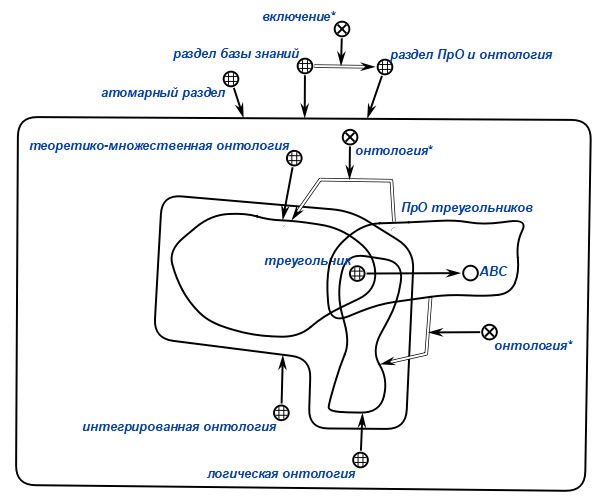
\includegraphics[scale=0.53]{figures/kb_develop_principles/example.png}
	\end{figure}
	
\end{frame}

\begin{frame}{\\Как ввести новую предметную область?}
	\topline
	\justifying
	\vspace{8mm}
	
\begin{textitemize}
	\item Определить ту (те) предметные области верхнего уровня, для которой она будет частной (по двум признакам: класс объектов исследования и по исследуемым отношениям).
	\item Разработать структурную спецификацию. 
	\item Разработать систему понятий. 
	\item Разработать примеры.
\end{textitemize}
\bigskip
Как правило разрабатываются (вводятся) явно:
\begin{textitemize}
	\item Предметная область и её структурная спецификация.
	\item Раздел предметная область и онтология (и его содержимое). 
\end{textitemize}

\end{frame}


\begin{frame}{\\Как ввести новое понятие?}
	\topline
	\justifying
	\vspace{8mm}
	
	\begin{textitemize}
		\item Определить ближайший надкласс (ближайшее более общее понятие). 
		\item Определить предметную область для этого понятия (возможно, ввести новую). 
		\item Разработать терминологическую онтологию. 
		\item Разработать теоретико-множественную онтологию.
		\item Разработать логическую онтологию (как естественным текстом, так и при помощи языка SCL).
	\end{textitemize}
	
\end{frame}



